\documentclass[times, utf8, diplomski]{fer}
\usepackage{booktabs}
\usepackage[final]{pdfpages}

\begin{document}

% TODO: Navedite broj rada.
\thesisnumber{2345}

\title{Proceduralno generiranje trave i niskog raslinja}
\author{Mihael Međan}

\maketitle

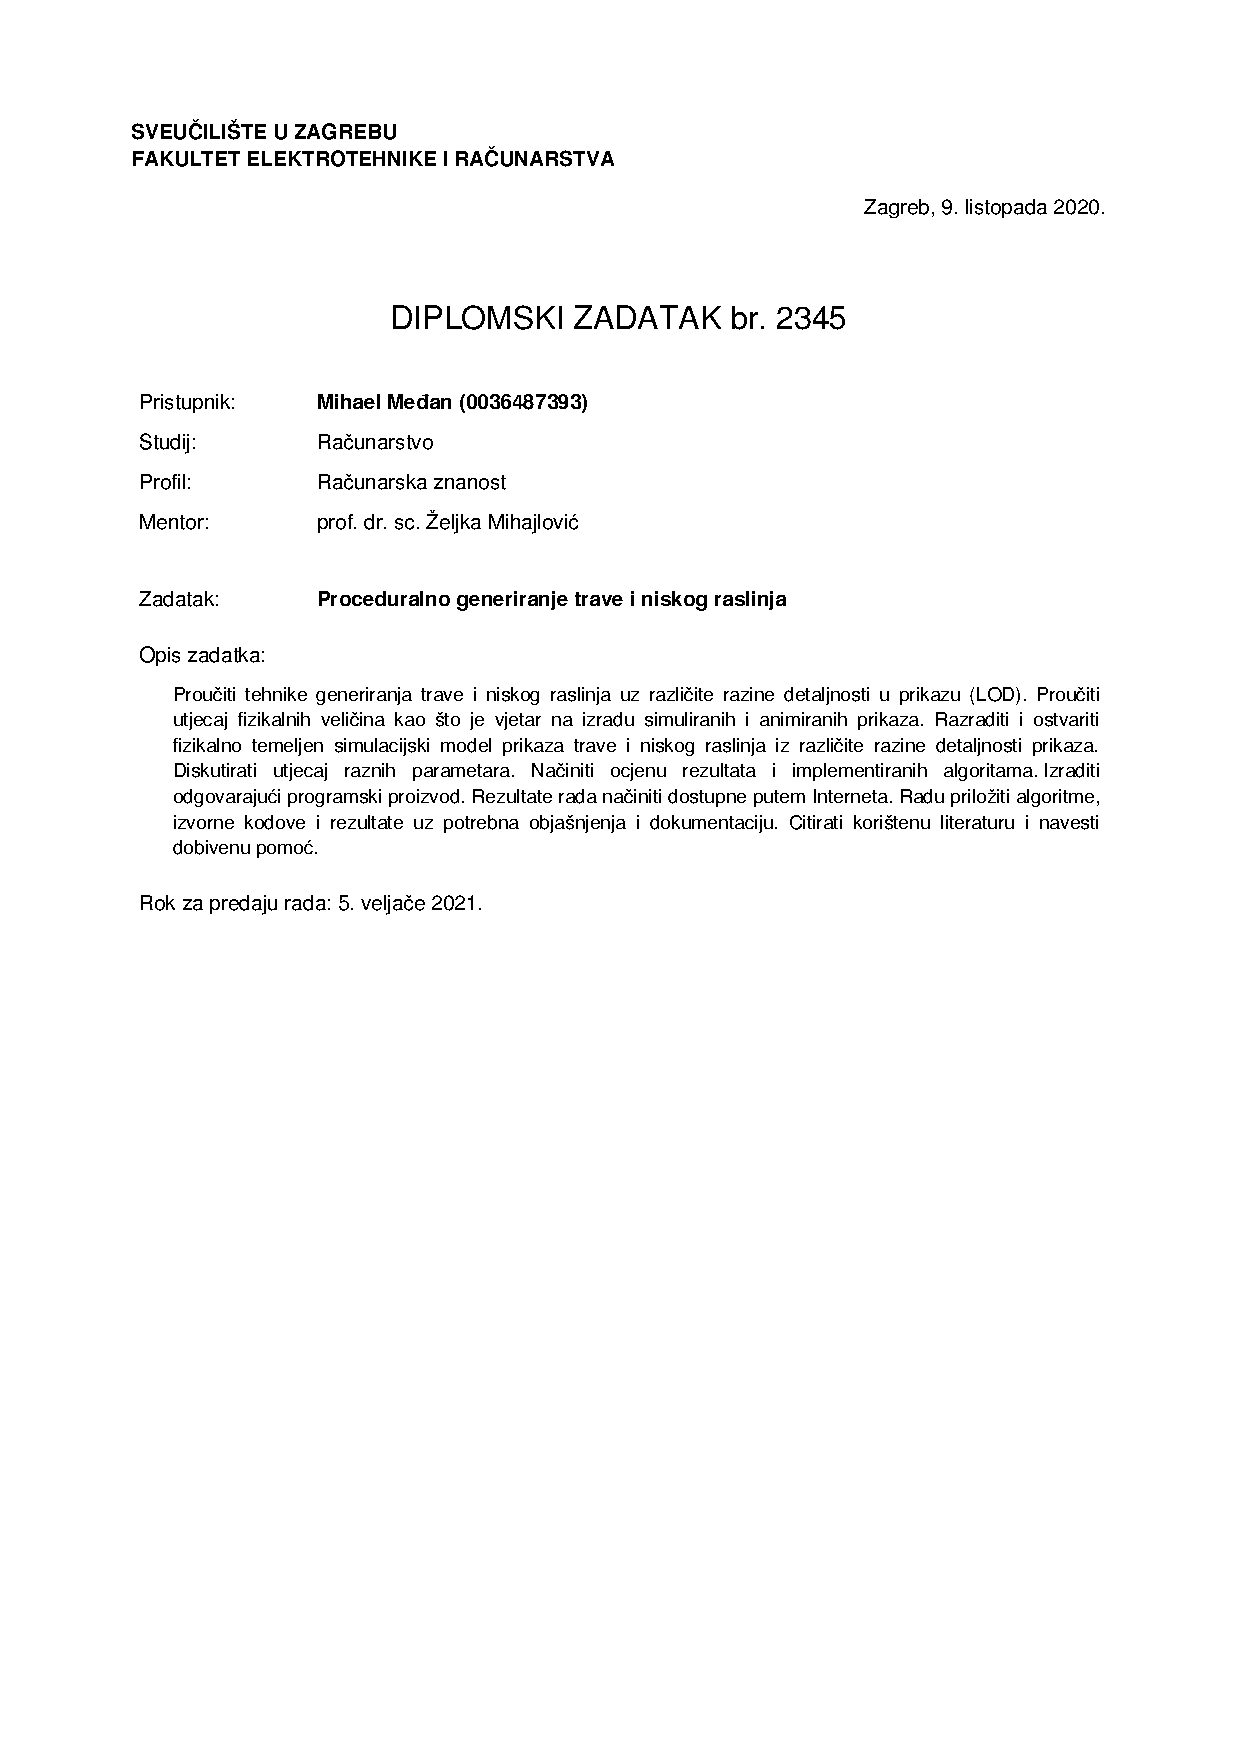
\includepdf[pages=-,offset=0 -75]{hr_0036487393_56.pdf}

\zahvala{}

\tableofcontents

\chapter{Uvod}
Uvod rada. Nakon uvoda dolaze poglavlja u kojima se obrađuje tema.

\chapter{Generiranje modela trave i niskog raslinja}
\section{Osnovni pristup generiranju modela}


\section{Generiranje točaka i poligona modela biljaka}
Tocke i poligoni

\subsection{Generiranje modela uz različitu razinu detalja}
LOD

\section{Povezivanje generiranih podataka i njihov prikaz}
Povezivanje i prikaz

\section{Programska implementacija generiranja i prikaza}
Tehnicka implementacija

\section{Primjer korištenja razvijenog programa za generiranje jednostavne proizvoljne biljke}
Primjer

\section{Dodavanje proizvoljnih atributa generiranim modelima}
Primjer

\section{Smjer implementacije generiranja složenijih biljaka}
Wish do, would do, not :)

\chapter{Simulacijski model}
\section{Fizički model ponašanja biljke}
Kako bi se biljka kretala hehe

\section{Programski model fizičkog ponašanja}
Pojednostavljenje na jointove etc

\section{Programska implementacija fizičkog modela}
EZ

\section{Smjer implementacije fizičkog ponašanja složenijih biljaka}
drva buraz e

\chapter{Simulacija ponašanja generiranog modela}
\section{Povezivanje fizičkog modela sa generiranim prikazom modela}
skinning, buffers, bones

\section{Programska implementacija modela}
spajanje

\section{Utjecaj parametara na simulaciju}
wind, elasticity

\chapter{Ocjena rezultata}
\section{Realističnost prikaza}
bad
\subsection{Poboljšanje realističnosti prikaza}
easy

\section{Realističnost fizičke simulacije}
good

\subsection{Poboljšanje realističnosti simulacije}
better

\section{Ocjena brzine izvođenja}
meh

\subsection{Pristupi poboljšanju brzine izvođenja}
\subsubsection{Paralelno izvođenje fizičke simulacije}
paralelism

\subsubsection{Smanjenje rezolucije simulacije i interpolacija rezultata}
nice

\subsubsection{Izračunavanje sličnosti modela i grupiranje izračuna}
bad

\chapter{Zaključak}
ma moze se sve buraz kad se oce

\bibliography{literatura}
\bibliographystyle{fer}

\begin{sazetak}
Sažetak na hrvatskom jeziku.

\kljucnerijeci{Ključne riječi, odvojene zarezima.}
\end{sazetak}

% TODO: Navedite naslov na engleskom jeziku.
\engtitle{Procedural generation of grass and low vegetation}
\begin{abstract}
Abstract.

\keywords{Keywords.}
\end{abstract}

\end{document}
